
% this file is called up by thesis.tex
% content in this file will be fed into the main document

%: ----------------------- introduction file header -----------------------
\chapter{Research Objectives}\label{ch:hypothesis}

\graphicspath{{hypothesis/figures/}}

% -------------------------------------------------------------
% -- Research Objectives 
% -------------------------------------------------------------

The work presented in this thesis aims to facilitate the exploration of large collections of multilingual documents through thematic associations inferred from their content. Each of the challenges arising from this objective defines a working dimension and guides the research carried out in this thesis.

The first dimension focuses on \textbf{scalability}, in order to create the text processing flows that are required to create or apply learning models. The workload required to process a corpus varies according to the number of documents, the length of texts and the kind of knowledge (annotations) that need to be infer from the text. If the design of the workflow is scalable, there is no need to modify the processing logic when working with larger collections of documents, since adding a reasonable amount of computational resources is enough to perform it. These resources can be machines (i.e horizontal scaling) or processing units (e.g CPU, RAM) in an existing machine (i.e vertical scaling). 

The second dimension covers the \textbf{representativeness} of the text annotations when projected into spaces where they are manipulated. The idea behind these spaces is to represent documents as points ( or vectors in a vector space) that are close together when the texts are semantically similar, and far apart when they are semantically distant. The ability of these spaces to create meaningful representations is studied in this work.

In the third dimension, data structures that efficiently \textbf{sorting} texts from their representations based on probabilistic topics were studied. Divisions of space into semantically-related regions are necessary to allow browsing large document collections. The \textit{representativeness} covered in the previous dimension enables the interpretation of the relations and regions obtained.

And finally, the fourth dimension handles the \textbf{multilingualism} of collections that contain documents in several languages. On a multilingual space, documents are described and related across languages.

This chapter introduces our main hypothesis (\ref{sec:research-hypothesis}), its associated research challenges (\ref{sec:research-challenges}) and presents the research methodology (\ref{sec:research-methodology}).

\section{Research Hypotheses}\label{sec:research-hypothesis}

We define our main hypothesis as follows:

\textbf{Hypothesis 1} \textit{Large multilingual document collections can be automatically analyzed to discover appropriate thematic relations that facilitate a semantically-enabled text browsing}.

Our hypothesis can be divided into four different sub-parts, which are related to the aforementioned scalability, representativeness, sorting, and multilinguality dimensions respectively. First, by \textit{distributing both natural language processing tasks and representational models we can efficiently process big collections of documents(\textbf{H1.1})}.

Second, we can \textit{semantically relate documents by comparing their most relevant topics (\textbf{H1.2})}. Furthermore, for this purpose we hypothesize that the use of \textit{topic hierarchies (\textbf{H1.2.1}) and similarity metrics based on relevance levels(\textbf{H1.2.2}) can help quantifying the semantic distance between texts}. Third, by \textit{dividing the representational space into regions based on topics and relevance levels we can search for related documents without having to calculate all pairwise comparisons and without losing the ability to rely on topics for further processing down the line (\textbf{H1.3})}.

And finally, \textit{by abstracting the topic representations into concept-based descriptions across languages we can relate documents in various languages without having to translate them (\textbf{H1.5})}.

A summary of the hypotheses and how they tackle our research objectives can be found in Table~\ref{table:hypotheses}.

\begin{table}[!htbp]
\centering%
\begin{tabularx}{\linewidth}{bs}
\toprule
\heading{Hypothesis} & \heading{Research Dimension } \\
\midrule
\midrule
H1: Large multilingual document collections can be automatically analyzed to be semantically-browsed through thematic relations & D1: Scalability, D2: Representativeness, D3: Sorting, D4: Multilingualism \\
\midrule
H1.1: it is possible to efficiently annotate documents on a large scale by distributing natural language processing tasks and representation models & D1: Scalability\\
\midrule
H1.2: it is possible to semantically relate texts from their most relevant topics & D2: Representativeness\\
\midrule
H1.3: it is possible to find documents with similar topic distributions without calculate all pairwise comparisons and without losing the ability to explore them through their topics & D3: Sorting\\
\midrule
H1.4: it is possible to relate documents in different languages without having to translate them using language agnostic concepts from their main topics & D4: Multilingualism\\
\bottomrule
\end{tabularx}
\caption{Hypotheses and research dimensions.}
\label{table:hypotheses}
\end{table}


\section{Research Challenges}\label{sec:research-challenges}

Several research challenges emerge from these hypotheses. First, in order to facilitate reusing existing topic models by processing systems with different architectures and technological stacks, we need to define \textit{topic-model programming interfaces}. Second, in order to describe and thematically relate documents, we must address how to produce \textit{explainable topic-based associations}. Third, by working with huge collections of documents described by topics, we need to handle \textit{large-scale comparisons of topic distributions}. Finally, in order to explore multilingual document collections from shared topic-based representational spaces, we have to provide \textit{automatic cross-lingual topic alignment}. Each of these research challenges are described below and covered throughout this thesis.

\subsection{Topic-model Programming Interface}

Although some initiatives to standardize the format of machine-learning models and to provide tools that facilitate their transformation among the most widespread proprietary formats already exist in the literature, there are still some software restrictions that can limit their reuse. These models may hold certain software dependencies that e.g. force using a specific version of a programming language (python2 vs python3\footnote{\url{https://www.python.org}}) or an operating system (e.g., linux kernel vs on-cloud environments\footnote{\url{https://vespa.ai}}) to load them or to launch the service that deploys them (e.g., ONNX\footnote{\url{https://onnx.ai}}). This limits their ability to be reused in domains that are not familiar with these technological stacks. \textit{Integrating pre-trained topic models into general-purpose systems is not easy \textbf{(RCInterface1)}}.


Topic models, as many other machine learning models, may be distributed in a proprietary or standard format with software dependencies or by directly providing the data. However, \textit{there is no standard way to specify the topics and the operations that can be performed on them \textbf{(RCInterface2)}}. Sometimes topics are described by the top ten or five most relevant words, and occasionally these word lists are not accompanied by weights, making a density-based analysis impossible. These differences in presenting the models can sometimes limit their reusability if they cannot infer new topic distributions even when the learning algorithm allows it.


\subsection{Explainable Topic-based Associations}

In order to facilitate the exploration of document collections, vector space models are often used to semantically relate texts based on their word distributions. These models first create a dictionary with the words used in the collection, and then represent  documents by vectors whose dimensions correspond to each word in the dictionary. In large collections, these models need to be adapted to make operations on vectors more manageable. As a result, a new abstraction method based on topics emerged that reduces the dimensions of vectors. Topics are described by word distributions over the entire vocabulary and documents by vectors containing topic distributions. Despite the extensive use of these representation models, \textit{there is no common criteria for identifying the most representative topics in a document \textbf{(RCExplainable1)}}. 

In addition, since similarity metrics over this representation space are based on accumulating the difference in topic densities, \textit{it is difficult to explain the distance between topic distributions \textbf{(RCExplainable2)}}. And, unless a minimum distance threshold is defined or a n-top topics agreed, \textit{there is no common criterion for determining whether two documents are related\textbf{(RCExplainable3)}}.  


\subsection{Large-scale Comparisons of Topic Distributions}

There are many scenarios where finding related documents in a large corpus is desirable (e.g. a researcher doing literature review, or an R\&D  manager analyzing project proposals). Experts can benefit from discovering those connections to achieve these goals, but brute-force pairwise comparisons are not computationally adequate when the size of the corpus is too large. Some algorithms in the literature divide the search space into regions containing potentially similar documents, which are later processed separately from the rest in order to reduce the number of pairs compared. However, \textit{there are no mechanisms that efficiently partition the topic-based search space without compromising the ability for thematic exploration \textbf{(RCComparison1)}}.

In addition, documents from the same region should be compared and \textit{there are no similarity metrics that compare partial distributions of topics \textbf{(RCComparison2)}}.


\subsection{Automatic Cross-lingual Topic Alignment}

With the ongoing growth in the number of digital articles in different languages, we need annotation methods that enable browsing multi-lingual corpora. Multilingual probabilistic topic models have recently emerged as a group of semi-supervised machine learning models that can be used to perform thematic explorations on collections of texts in multiple languages. However, \textit{there are no approaches that abstract the representation of probabilistic topics in language-independent spaces without translating texts or aligning documents\textbf{(RCCrossLingual1)}}. Existing approaches require parallel or comparable training data to create a language-independent space. 

A summary of the challenges covered in this work and how they map to the hypotheses is presented in table\ref{table:challenges}

\begin{table}[!htbp]
\small
\centering%
\begin{tabularx}{\linewidth}{bb}
\toprule
\heading{Research Challenge} & \heading{Hypotheses} \\
\midrule
\midrule
RCInterface1: integrating pre-trained topic models into general-purpose systems is not easy & H1.1: documents can be efficiently annotated on a large scale by distributing natural language processing tasks and representation models\\
\midrule
RCInterface2: there is no standard presentation of topics that facilitates their reuse & H1.1: documents can be efficiently annotated on a large scale by distributing natural language processing tasks and representation models\\
\midrule
RCExplainable1: there is no common criteria for identifying the most representative topics in a document & H1.2: texts can be semantically related from their most relevant topics, H1.3: documents with similar topic distributions can be found without calculate all pairwise comparisons and without losing the ability to explore them through their topics \\
\midrule
RCExplainable2: it is difficult to understand the distance between topic distributions & H1.2: texts can be semantically related from their most relevant topics\\
\midrule
RCExplainable3: there is no common criterion for determining whether documents are related & H1.2: texts can be semantically related from their most relevant topics\\
\midrule
RCComparison1: there are no mechanisms that efficiently partition the topic-based search space without compromising the ability for thematic exploration & H1.3: documents with similar topic distributions can be found without calculate all pairwise comparisons\\
\midrule
RCComparison2: there are no similarity metrics that compare partial distributions of topics & H1.3: documents with similar topic distributions can be found without calculate all pairwise comparisons\\
\midrule
RCCrossLingual1: there are no approaches to abstract probabilistic topics in language-independent spaces without translating texts or aligning documents  & H1.4: documents in different languages can be related without having to translate them using language agnostic concepts from their main topics\\
\bottomrule
\end{tabularx}
\caption{Open Research Challenges and Hypotheses.}
\label{table:challenges}
\end{table}

\section{Research Methodology}\label{sec:research-methodology}

The research presented in this thesis is based on four dimensions or research areas. Each one is motivated by different research problems that we need to solve in order to achieve our ultimate goal of making it easier to explore large multilingual document collections through their topics. Once a dimension is tackled, the next one is considered, and so on. This iterative and incremental methodology allows us refining the research results by evaluating them with more experiments and addressing increasingly complex research problems.

Figure \ref{fig:dimensions} shows the dimensions on which the research of this thesis has been built. The top of the pyramid is only reached once the lower dimensions are dealt with. They are presented as a chain of four steps. The first step describes the motivation to perform a given task coming from real-world problems that we had to deal with and is represented by a brown arrow. In the context of this task, the research problem arises and is framed by a pink arrow. For each of them a solution is proposed and evaluated according to a specific criterion. The proposed solution is represented by a green arrow and the evaluation with a blue arrow. Once a proposal has been validated, the next dimension of the pyramid is achievable and all the previous research problems are added to the new research problem as conditions to be taken into account

Technical objectives (i.e., develop a new resource) or research objectives (i.e., discover the solution to a problem) guide the solution proposal before moving on to the next dimension. They are presented below, organized by the research problem associated with each dimension.


\subsection{Scalable Creation and Inference of Topics}

This first dimension arose when we had to analyze a huge collection of documents describing research and innovation projects to discover which research areas are being addressed, measure their presence in the collection, and characterize them so that they can be assigned to new documents. Such a high volume of data made difficult to process it manually, so we needed to automatize the required processing to draw insights from it. Probabilistic topics allow describing research areas, so we defined a \textit{distributed text-processing model for creating large probabilistic topic models (\textbf{RO1})} and a \textit{web service template to distribute them (\textbf{RO2})}. In this way, the models themselves could be easily integrated into scalable processing pipelines. As a result, we created a \textit{platform for large-scale text analysis (\textbf{TO1})}, and produced a \textit{model-as-a-service repository with pre-trained topic models(\textbf{T02})}. The efficiency of this solution was validated by processing a corpus of 100,000 documents collected from the CORDIS dataset\footnote{\url{https://data.europa.eu/euodp/es/data/dataset/cordisH2020projects}}, which contains descriptions of projects funded by the European Union under a framework programme since 1990 \citep{Badenes-Olmedo2017}. 

The main contributions under this dimension are described in Section \ref{ch:scalability} as follows:
\begin{itemize}
\item a software architecture to process big volumes of textual documents in a distributed and decoupled manner;
\item the definition of a model-as-a-service template for probabilistic topic models;
\item an implementation of the architecture, librAIry, following those design principles;
\end{itemize} 


\subsection{Explainable Topic-based Associations}

In the second dimension we needed to browse scientific papers through their content-based relations. The problem of massively annotating documents with topic distributions came up. We had to \textit{create annotations based on topic models in a way that was computationally affordable and enabled a semantic-aware exploration of the knowledge inside it (\textbf{RO3})}. Once documents were annotated, a \textit{metric that compares documents and facilitates their interpretation from topic annotations (\textbf{RO4})} was required. As a result, we integrated \textit{the annotation method into the topic model service (\textbf{TO3})} and implemented a text comparison metric based on partial representations of topics. These proposals were validated by classifying 500,000 scientific articles from Open Research Corpus\footnote{\url{https://allenai.org/data/open-research-corpus}} in domains such as Computer Science, Neuroscience and Biomedicine \citep{Badenes-Olmedo2017b} \citep{Badenes-Olmedo2017c} \citep{Badenes-Olmedo2019b}. 

The main contributions under this dimension are described in Section \ref{ch:explainability} as follows:
\begin{itemize}
\item a clustering algorithm based on probabilistic topic distributions;
\item a hash function to transform topic distributions into topic hierarchies;
\item a similarity metric based on topic sets; 
\end{itemize} 

\begin{figure}[!htbp]
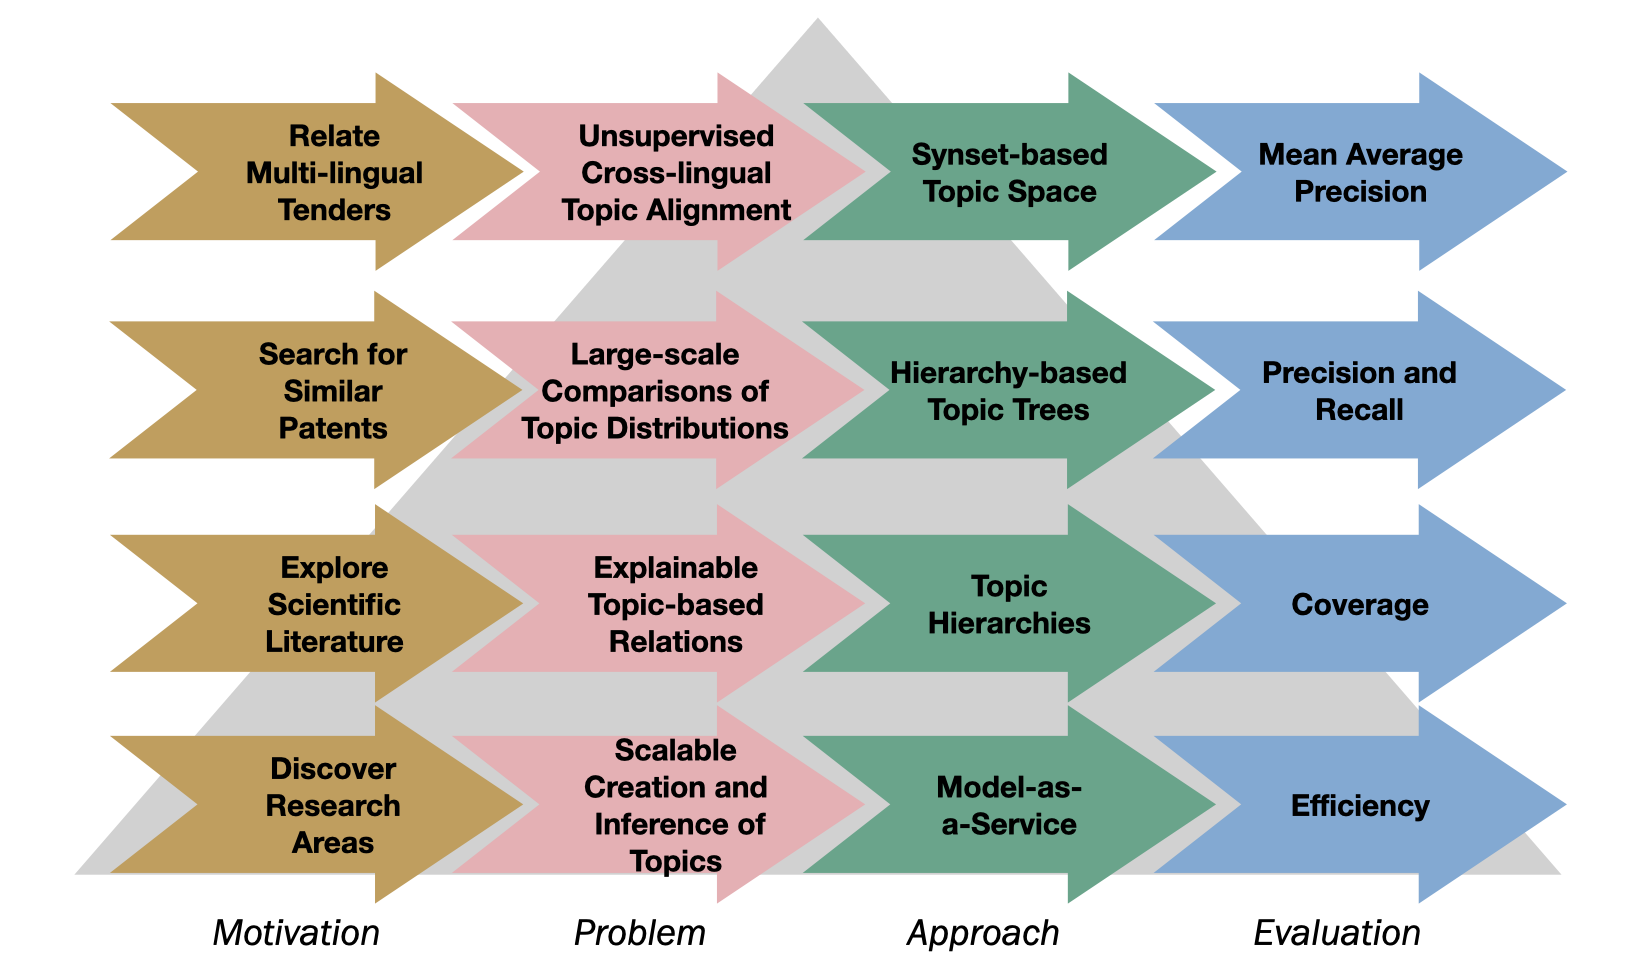
\includegraphics[scale=0.25]{dimensions.png}
\centering
\caption{Research dimensions of the thesis. The first ones must be overcome before reaching higher dimensions. }
\label{fig:dimensions}
\end{figure}

\subsection{Large-scale Comparisons of Topic Distributions}

This dimension covered the search for similar documents based on their most relevant topics. Thanks to the above two dimensions, large collections of documents could be annotated with topic hierarchies and text distances could be measured from their annotations. Now, the aim was to find similar documents without losing the exploratory capacity offered by topics. Similarity comparisons were too costly to be performed in such huge collections of data and required more efficient approaches than having to calculate all pairwise similarities. We applied \textit{techniques based on approximate nearest-neighbors to organize documents in regions with similar topic hierarchies (\textbf{RO5})}. As a result, we developed \textit{a system to automatically find similar documents (\textbf{TO4})}. It was validated on a collection of one million texts retrieved from the United States patents corpus\footnote{\url{https://www.uspto.gov/ip-policy/economic-research/research-datasets}}. The relations between patents derived from their manual categorization were compared with those automatically obtained from their topic distributions \citep{Badenes-Olmedo2020}\citep{Badenes-Olmedo2019b}. 

The main contributions under this dimension are described in Section~\ref{ch:comparisons} as follows:
\begin{itemize}
\item a data structure to partition the search space and organize documents described by topic hierarchies
\item a corpus browser that leverages these representations to automatically relate documents
\end{itemize} 


\subsection{Automatic Cross-lingual Topic Alignment}

Finally, a new dimension on top of the previous ones emerged to relate texts coming from different languages. In particular, since document relations were based on their topics, this dimension was focused on aligning topics without supervision from models trained with texts in different languages. Since each language defined its own vocabulary, the topics were model-specific and could not be directly compared. We abstracted the \textit{topic representations to create a single space out of the particularities of the language (\textbf{RO6})}.This approach was validated on the English, Spanish, French, Italian and Portuguese editions of JCR-Acquis\footnote{\url{https://ec.europa.eu/jrc/en/language-technologies/jrc-acquis}} corpora and revealed promising results on classifying and sorting documents by similar content across languages \citep{Badenes-Olmedo2019}\citep{Badenes-Olmedo2019b}. 

The main contributions under this dimension are described in Section~\ref{ch:multilinguality}, as follows: 
\begin{itemize}
\item an algorithm to represent probabilistic topics using concept sets
\item a repository of aligned topic models from the English, Spanish, French, Italian and Portuguese editions of the JRC-Acquis corpus
\end{itemize}

Table \ref{table:objectives} summarizes the research objectives (ROs), technical objectives (TOs) and connects them with the research challenges (RCs) from Table \ref{table:challenges}.


\begin{table}[!htbp]
\centering%
\small
\begin{tabularx}{\linewidth}{bs}
\toprule
\heading{Research Objective} & \heading{Research Challenge}\\
\midrule
\midrule
RO1: Define a distributed text-processing model for creating large probabilistic topic models  & RCInterface1 \\
\midrule
RO2: Define a template to package probabilistic topic models as web services & RCInterface2\\
\midrule
RO3: Define annotations based on topics that enables a semantic-aware exploration of the knowledge inside a corpus & RCExplainable1\\
\midrule
R04: Define a metric based on topic annotations that compares documents and facilitates their interpretation & RCExplainable2, RCExplainable3\\
\midrule
RO5: Define nearest-neighbors techniques to organize documents in regions with similar topic hierarchies & RCComparison1, RCComparison2\\
\midrule
R06: Define a transformation of the topic-based annotations to create a unique representational space out of the particularities from each language & RCCrossLingual1\\
\midrule
TO1: Create a platform for large scale text processing & RCInterface1, RCInterface2\\
\midrule
T02: Create a repository of Topic-based web services & RCInterface2\\
\midrule
T03: Integrate the annotation method based on topic hierarchies into the topic model service & RCExplainable2, RCComparison2\\
\midrule
T04: Create a system capable of finding similar document automatically & RCExplainable2, RCExplainable3, RCComparison1, RCCrossLingual1\\
\bottomrule
\end{tabularx}
\caption{Research and technical objectives and their related challenges.}
\label{table:objectives}
\end{table}
